\subsection{Configure Data Sources}
\label{sec:ui_configure_data_sources}

This dialog allows management of data sources, as stored in the configuration as well as the database. \\

\begin{figure}[H]
  \center
    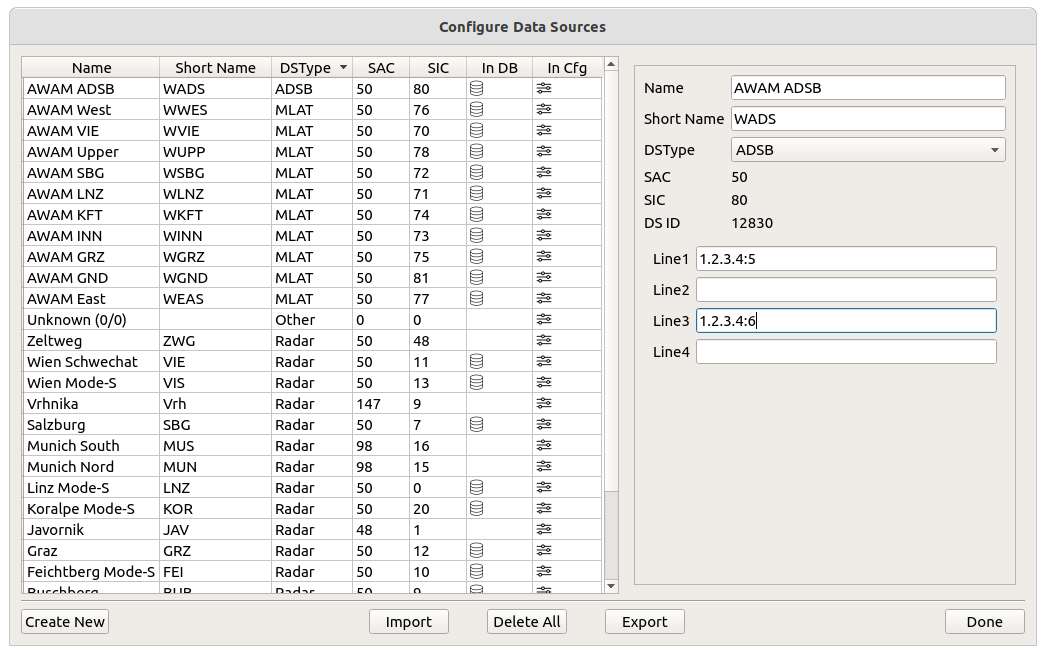
\includegraphics[width=16cm]{figures/configure_data_sources.png}
  \caption{Configure Data Sources}
\end{figure}

If data is imported from ASTERIX, data source information might be missing, so this information must either be edited manually, or loaded from a previous configuration (or previous database containing the same information). \\

A data source is always stored in the configuration, which means it is persisted and can be used in all new databases. It is useful to define all existing data sources in the configuration, since they are immediately used during import of data. \\

A data source is stored in the database only if data from said source is imported. During the import, if a data source can be found (matching SAC/SIC) in the configuration, it is automatically added to the database. \\

Please \textbf{note} that currently the position of data sources is only required for \textbf{Radar} data sources (in the plot position calculation), for the others it would suffice to have SAC/SIC and name information for display purposes.

\paragraph {Data Sources Table Content}
\label{sec:configure_datasources_table_content}

\begin{itemize}
\item Name: Name of the data source
\item Short Name: Short name of the data source (optional)
\item DSType: Data source type, e.g. Radar, MLAT, ADS-B, ...
\item SAC: System Area Code, number between [0,255]
\item SIC: System Identification Code, number between [0,255]
\item In DB: Indicator whether the data source is stored in the database
\item In Config: Indicator whether the data source is stored in the configuration
\end{itemize}
\ \\

When a data source is selected in the table, additional details are shown in the right side, where edting is also possible. \\

Please \textbf{note} that all changes to a data sources are always written to the database as well as the configuration. \\

Depending on the DSType, additional information can be set in a source. For a non-Radar source, the following information is given:

\begin{itemize}
\item ID: Number indentifier (unique)
\item Network Line information
\begin{itemize}
    \item 4 different lines are possible, each with an 'IP:Port' syntax
\end{itemize}
\end{itemize}
\ \\

For sources of DSType Radar, the follwing additional information can be given:

\begin{itemize}
\item Latitude: Source center position as WGS-84 latitude, as floating point number in degrees, e.g. 42.0001
\item Longitude: Source center position as WGS-84 longitude, as floating point number in degrees, e.g. 17.01
\item Altitude: Source center altitude above MSL, in meters
\end{itemize}
\ \\

Additional optional information can be given:

\begin{figure}[H]
  \center
    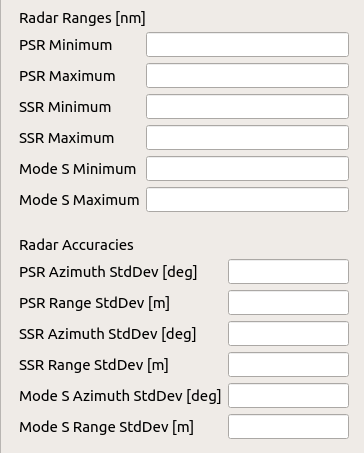
\includegraphics[width=8cm,frame]{figures/configure_data_sources_radar_details.png}
  \caption{Configure Data Sources: Radar details}
\end{figure}

\begin{itemize}
\item PSR Minimum: PSR minimum range, in nautical miles
\item PSR Maxmimum: PSR maximum range, in nautical miles
\item SSR Minimum: SSR minimum range, in nautical miles
\item SSR Maxmimum: SSR maximum range, in nautical miles
\item Mode S Minimum: Mode S minimum range, in nautical miles
\item Mode S Maxmimum: Mode S maximum range, in nautical miles
\item PSR Azimuth StdDev: PSR azimuth standard deviation, in degrees
\item PSR Range StdDev: PSR range standard deviation, in meters
\item SSR Azimuth StdDev: SSR azimuth standard deviation, in degrees
\item SSR Range StdDev: SSR range standard deviation, in meters
\item Mode S Azimuth StdDev: Mode S Radar azimuth standard deviation, in degrees
\item Mode S Range StdDev: Mode S Radar range standard deviation, in meters
\end{itemize}
\ \\

\subsection{Import/Export of Configuration Data Sources}
\label{sec:config_ds_export}

Using the 4 buttons on the bottom the following functions can be used:

\begin{itemize}
\item Export All: Export all configuration data sources from all DBObjects as JSON file
\item Clear All: Delete all configuration data sources from all DBObjects
\item Import: Import configuration data sources for all DBObjects from JSON file
\item Auto Sync All to DB: Automatically synchronize all configuration data sources to database
\end{itemize}
\ \\

There are two versions of the data sources JSON file used for import/export. Please refer to \nameref{sec:appendix_data_sources}. \\

Using these functions, the configuration data sources can be changed for sensor context switches, or e.g. exported before an COMPASS version upgrade.
